\documentclass[a4paper,11pt]{article}
\usepackage{graphicx}
\usepackage{caption}
\usepackage{vub} % Keeps your university formatting
\usepackage{listings}
\usepackage{hyperref}
\usepackage{tabularx}
\usepackage{booktabs}
\usepackage{float}
\usepackage{subcaption}
\usepackage{cite}
\usepackage{amsmath}

% --- TITLE SETUP ---
\title{Image Super-Resolution}
\subtitle{Deep Learning Project Report}
\date{24 August 2026}
\faculty{MACS}
\author{
Jawad Shaissah \\
Hamed Nikoo \\
Fahimeh Safari Moghadam
}

% --- float placement: allow figures to share pages with body text ---
\renewcommand{\topfraction}{0.92}
\renewcommand{\bottomfraction}{0.85}
\renewcommand{\textfraction}{0.06}
\renewcommand{\floatpagefraction}{0.80}
\setcounter{topnumber}{3}
\setcounter{bottomnumber}{2}
\setcounter{totalnumber}{4}

\begin{document}
\maketitle

% --- TABLE OF CONTENTS ---
\tableofcontents
\newpage


% ==================================================================
% 1. INTRODUCTION AND MOTIVATION
% ==================================================================
\section{Introduction and Motivation}

Single-image Super-resolution is the task of upscaling a low-resolution image into a higher-resolution one, without losing details or introducing artefacts such as in classical methods (e.g., bicubic). Enhancing the resolution of an image from low-resolution (LR) to high resolution (HR) matters in applications such as surveillance cameras and in image and video compression.

\medskip

In this project, we focus on learning-based super-resolution methods and implement a deep neural network to upscale images by a factor of $\times 4$, following the project guidelines. We use the DIV2K dataset, where low-resolution images are generated using bicubic downsampling, and train the model on image patches rather than full images to increase the number of training samples and improve generalization. After holding out 10 images for validation, training runs on the remaining 790. 

\medskip

We implement the Enhanced Deep Residual Network (EDSR) architecture, which processes the low-resolution input directly and performs upsampling. The model learns to reconstruct high-frequency details from data. Our main objective is to correctly implement the full training and evaluation pipeline and analyze the effect of the model on both quantitative metrics and visual quality.

We chose this task because, unlike classification, it requires the model to produce an entire
image as output, which makes it far more sensitive to architectural choices and to how carefully
the results are measured. That sensitivity is the subject of this report.

% ==================================================================
% 2. BRIEF LITERATURE REVIEW
% ==================================================================
\section{Brief Literature Review}

To better understand our approach, it is useful to review the evolution of image super-resolution methods.

\subsection{Interpolation Methods (The Baseline)}
One of the most traditional approaches to image upscaling is bicubic interpolation.
This method estimates the value of a new pixel by computing a weighted average of its
16 nearest pixels in the low-resolution image.

\medskip


The main advantage of bicubic interpolation is its low computational cost, which allows
it to run efficiently in real-time on almost any device. However, since this method only
uses the existing pixel values, it is unable to generate new high-frequency details. As a
result, the upscale images often appear overly smooth, with blurred edges and missing
textures.

\medskip


In this project, we use bicubic interpolation as a baseline method to quantitatively and
qualitatively evaluate the improvement achieved by learning-based super-resolution
models.

\subsection{Early Deep Learning (SRCNN)}
The field of single image super-resolution changed significantly with the introduction of the
\textbf{Super-Resolution Convolutional Neural Network (SRCNN)} by Dong et al.~\cite{dong2014}.
This was one of the first methods to use a convolutional neural network to directly learn the mapping from low-resolution images to high-resolution images.

\medskip



Although SRCNN demonstrated that deep learning models could outperform classical interpolation methods, it had an important limitation. The low-resolution image first needed to be upscaled using bicubic interpolation before being passed to the network. This increased the computational cost, as the network had to process high-resolution feature maps, making the approach slower and less efficient.



Two further methods appear in our results table as baselines. A+~\cite{timofte2014} is the
strongest of the pre-deep-learning approaches and works by matching each low-resolution patch
to an entry in a learned dictionary and applying a linear regressor attached to that entry.
VDSR~\cite{kim2016} stacks 20 convolutional layers and predicts only the difference between the
bicubic-upsampled input and the ground truth, which is easier to learn than the image itself.
Like SRCNN it still runs every layer at high resolution.

\subsection{State-of-the-Art (EDSR)}\label{sec:edsr}
Building on the idea of residual learning, Lim et al.\ proposed the Enhanced Deep
Residual Network (EDSR)~\cite{lim2017}. What they argued is that Batch Normalization,
standard in residual networks for image classification, is the wrong tool for
super-resolution.

The problem is what it normalizes away. Batch Normalization rescales each feature map to
zero mean and unit variance, which discards the absolute scale of the features. A
classifier does not care about that, since a cat is a cat whether the photo is bright or
dark. Here it matters, because what we are predicting \emph{is} pixel intensity, and the
range information the layer removes is the thing we are trying to reproduce. It also ties
each output to the other images in the batch, which is odd for a task where every image is
reconstructed on its own, and it behaves differently at test time because the layer then
uses statistics collected during training instead of statistics from the image in front of
it.

There is a practical cost as well. A Batch Normalization layer takes up roughly as much
memory as the convolution it follows. Dropping it left enough room to make the network
deeper and wider, and that extra capacity turned out to be worth more than the
normalization had been.

\medskip


By removing Batch Normalization layers, the authors were able to design a deeper
and wider network that produces more accurate and visually consistent high-resolution
images. Due to its strong performance and relatively simple design, EDSR has become
a commonly used architecture for image super-resolution and is the model selected
for this project.


% ==================================================================
% 3. METHODOLOGY AND MODEL DESCRIPTION
% ==================================================================
\section{Methodology and Model Description}

In this section, we describe the proposed super-resolution method and the architecture
of the implemented EDSR model. We also outline the training procedure and key
implementation details relevant to our experiments.

\subsection{Model Architecture (EDSR)}

The network has three components: a data normalization layer, a deep residual body that
extracts features at low resolution, and an upsampling module that raises the spatial resolution
by $\times4$ at the very end.

\begin{figure}[htbp]
    \centering
    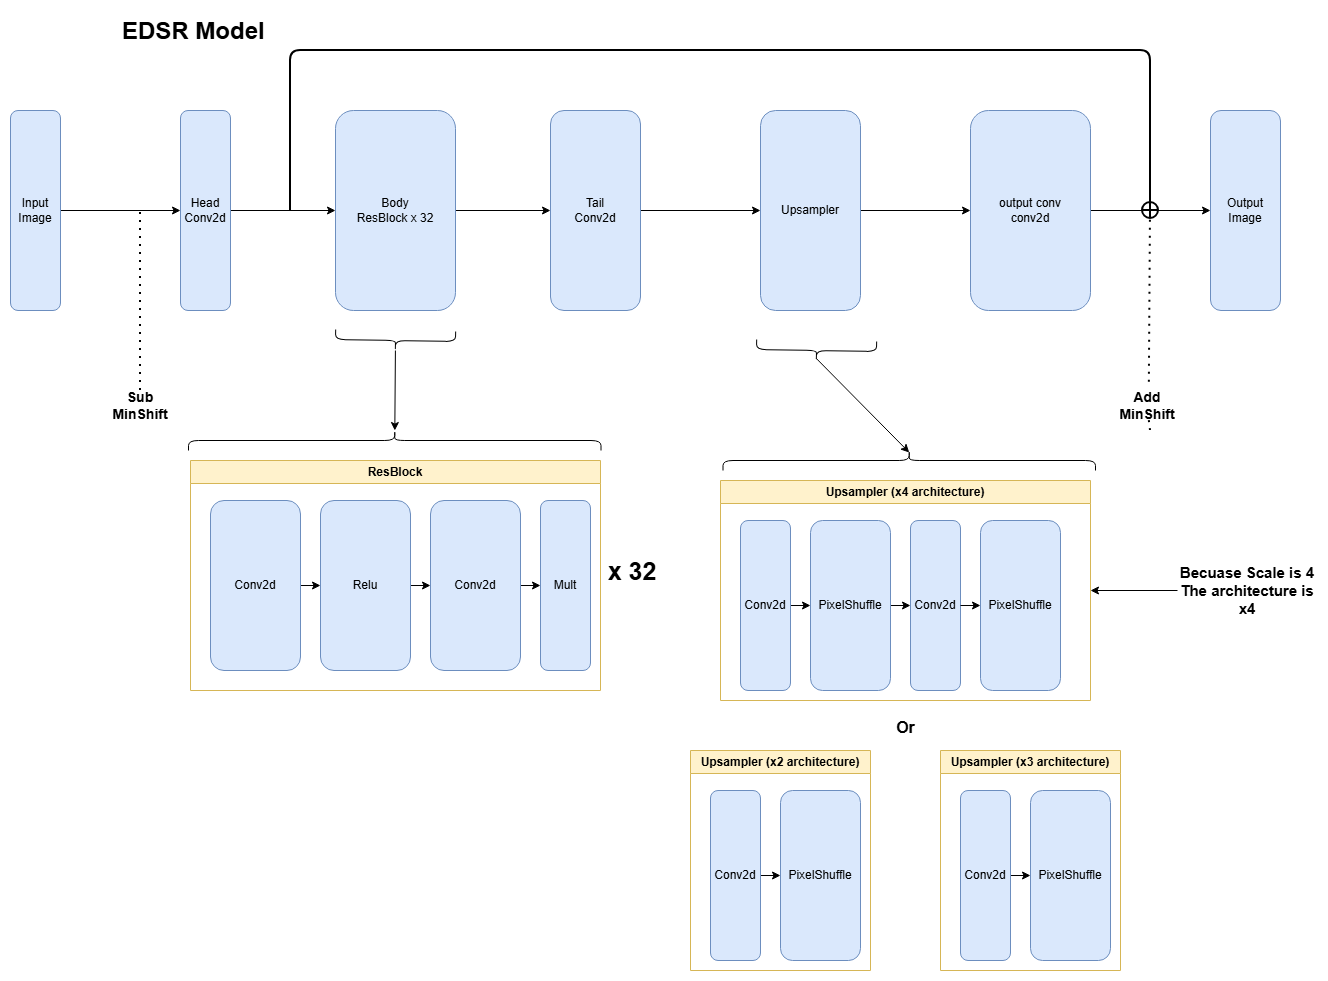
\includegraphics[width=0.50\linewidth]{img/model.drawio.png}
    \caption{EDSR Model}
    \label{fig:edsr_model}
\end{figure}


\subsubsection{Data Normalization (MeanShift)}

The input image is passed through a MeanShift layer. This
layer subtracts the average RGB values of the DIV2K dataset 
from the input image. By centering the data distribution around zero, the network can
focus on learning structural patterns such as edges and textures instead of adapting to
absolute brightness differences. This normalization helps stabilize training and leads to
faster convergence. The layer holds the channel means as fixed constants and is never trained.


\subsubsection{Residual Blocks (ResBlock)}
The core of the EDSR model is a deep stack of residual blocks used for feature
extraction. In our implementation, the network consists of 32 residual blocks, each
with 128 feature maps, allowing the model to learn rich image representations while
maintaining stable gradient flow through skip connections.

\medskip


Unlike standard residual blocks used in image classification, the Batch Normalization layers
are removed, for the reasons given in Section~\ref{sec:edsr}. Each block is therefore
convolution, ReLU, convolution, added to its own input.


\subsubsection{Upsampling Module (PixelShuffle)}

After feature extraction, the learned feature maps are passed to the upsampling
module. We use the PixelShuffle operation to increase the spatial resolution of the
image. Unlike transposed convolution layers, which can introduce checkerboard
artifacts, PixelShuffle rearranges feature maps to expand the height and width of the
image in a deterministic manner.

\medskip


This approach allows the network to perform the $\times4$ upscaling entirely at the end
of the model, as two successive $\times2$ PixelShuffle stages, resulting in efficient
computation and improved visual quality of the reconstructed high-resolution images.

\subsection{Training and Implementation Details}

The EDSR model was trained using a patch-based learning strategy to increase the
number of training samples and improve generalization. From each training image,
20 random low-resolution patches of size $48 \times 48$ were extracted per epoch.

\medskip


Training was performed using a batch size of 32 and optimized with the Adam
optimizer with an initial learning rate of $1 \times 10^{-4}$, halved at epochs
25 and 40 by a MultiStepLR schedule
($1 \times 10^{-4} \rightarrow 5 \times 10^{-5} \rightarrow 2.5 \times 10^{-5}$).
The network was trained for 100 epochs with the L1 loss as the objective
function, following the EDSR paper, which reports that it trains more stably and gives sharper
results than a squared error loss. We did not test this ourselves.
\medskip

Since the 100 DIV2K validation images are used as our test set, we could not
also use them to select the model. Instead, we held out 10 images from the
training set and used them for the per-epoch validation and checkpoint
selection (this is what Figure~\ref{fig:curves} shows). The test set was evaluated
only once, at the end, with the best checkpoint.
\subsection{Hardware and Experimental Setup}

All experiments were conducted on VUB GPU Farm (ETROFARM)  equipped
with CPU AMD EPYC 9124(F. 25 M.17), 2 sockets, 2x16x1= 32 (logical) CPU, 377GB, 4x Nvidia A100(Ampere) 80GB, Nvidia Driver: 535.247.01, CUDA 12.1.1. This hardware setup was sufficient to support patch-based training
with moderate batch sizes and allowed the EDSR model to be trained efficiently for
the required number of epochs. The same experimental setup was used consistently
across all experiments to ensure fair and reproducible results.

\subsection{Code Structure and Reproducibility}

The code is structured so that anyone can check our results or repeat them.

\medskip

The two evaluation functions from fix 3 are now one \texttt{evaluate} function that takes the
prediction routine as an argument. We push the model, the bicubic baseline and the self-ensemble
through it, so none of them can be scored differently by accident. We simplified the metric code
in the same pass. The old \texttt{PSNR} and \texttt{SSIM} classes are plain functions now
(\texttt{calc\_psnr}, \texttt{calc\_ssim}, \texttt{rgb\_to\_y}, \texttt{shave\_border}), and
the two luminance conversions that had drifted apart are a single function.

\medskip

The dataset comes from the four official DIV2K archives at ETH Zurich rather than a zip file on
someone's personal cloud drive, so anyone can get exactly the data we used. We seed every random
number generator from one value. That includes the dataloader workers, which previously inherited
the same seed and handed back correlated crops. The generator state also goes into the checkpoint,
so a resumed run continues the same sequence instead of starting a new one.

\medskip

The project also ships with the scripts we actually used. A smoke test runs the whole pipeline on
a handful of images in a few minutes, which catches shape and path errors before we queue a job
that takes hours. A second script runs the notebook end to end on the GPU farm and writes three
things into a per-run folder: the executed notebook, an HTML copy of it, and a record of the
software environment. Every number in this report has one of those folders behind it, so we can
point at the code that produced it and the package versions it ran against.


% ==================================================================
% 4. EXPERIMENTAL RESULTS
% ==================================================================
\section{Experimental Results and Discussion}

We evaluated the performance of our model using quantitative metrics and qualitative visual inspection.

\subsection{Testing Utilities}

We implemented three helper functions used during testing that help with evaluation.

\medskip


\textbf{Shave border.} When computing quantitative metrics, the outer pixels of the
output image may contain padding artifacts. Therefore, we cropped a border equal to the
scaling factor from both the prediction and the ground truth before evaluation, so that
PSNR, SSIM and LPIPS are all computed on exactly the same pixels.

\medskip


\textbf{Geometric ensemble.} We transform the input with the 8 symmetries of a square, pass each
version through the model, undo the transform on each output and average the 8 results. The model
is not exactly equivariant to rotation, so averaging cancels part of the disagreement between the
8 predictions, at the cost of 8 times the inference time. This is the
``EDSR + 8$\times$ self-ensemble'' row in Table~\ref{tab:final_results}.


\textbf{MATLAB-compatible bicubic resize.} The DIV2K low-resolution images were produced with
MATLAB's \texttt{imresize}, whose cubic kernel uses the Keys parameter $a=-0.5$ and applies
antialiasing when downscaling. PyTorch's bicubic interpolation uses $a=-0.75$ and no antialiasing, so
it is not the inverse of the degradation that created the dataset. We therefore implemented the
MATLAB version ourselves. A resize is a linear and separable operation, so we build the interpolation
weights as one matrix per axis and apply them to rows and then to columns. This function produces the
Bicubic row of Table \ref{tab:final_results}.

\subsection{Quantitative Analysis}
Here we present the evaluation of training stability, measured through the L1 loss used as the
training objective, followed by final performance on the three metrics required for this project:
Peak Signal-to-Noise Ratio (PSNR), Structural Similarity (SSIM) and Learned Perceptual Image Patch
Similarity (LPIPS).

\subsubsection{Training Curves}
The model was optimized using \textbf{L1 Loss} (Mean Absolute Error). As shown in
Figure~\ref{fig:curves}a, the loss decreased steadily over the 100 epochs, indicating that the
network converged without divergence. In parallel we monitored the \textbf{PSNR} on the 10-image
validation set held out of the training pool (Figure~\ref{fig:curves}b); it improves rapidly during
the early epochs and continues to gain marginal improvements toward the end of training.

\begin{figure}[htbp]
    \centering
    \begin{subfigure}[t]{0.48\textwidth}
        \centering
        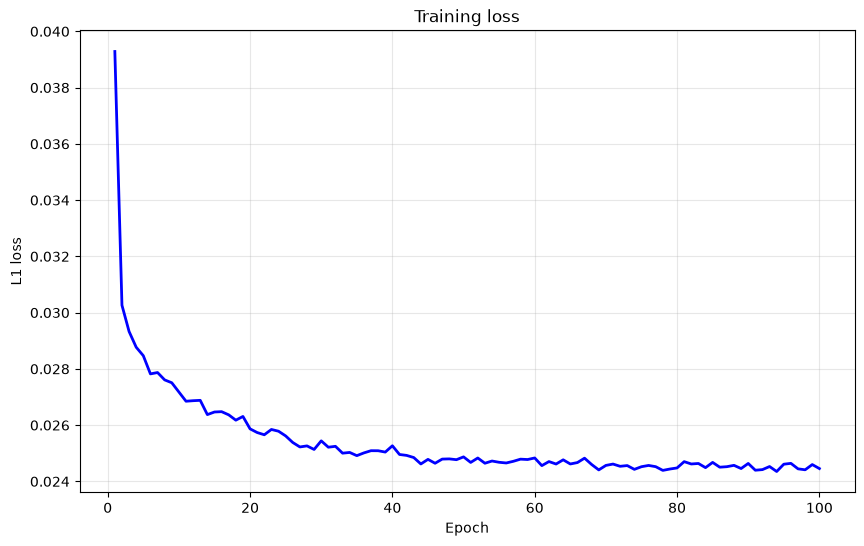
\includegraphics[width=\linewidth]{./newimg/l1_loss_plot.png}
        \caption{L1 training loss.}
    \end{subfigure}\hfill
    \begin{subfigure}[t]{0.48\textwidth}
        \centering
        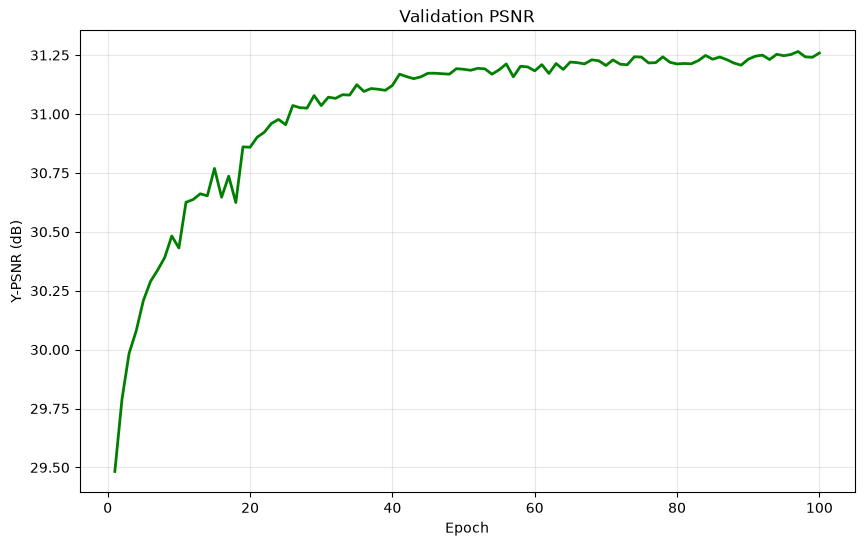
\includegraphics[width=\linewidth]{./newimg/psnr_plot.png}
        \caption{Validation PSNR.}
    \end{subfigure}
    \caption{\textbf{Training curves over 100 epochs.} (a) The training loss shows a consistent
    downward trend, confirming effective learning without divergence. (b) The validation PSNR
    increases steadily, reaching a peak of 31.27~dB. This curve is measured on the 10 images held
    out of the training pool for checkpoint selection, not on the test set, which is why it sits
    above the 30.41~dB reported in Table~\ref{tab:final_results}: the validation set is both smaller
    and the set the checkpoint was chosen on. The gap is expected once selection and reporting are
    separated.}
    \label{fig:curves}
\end{figure}

\subsubsection{Final Quantitative Evaluation}
We evaluated our proposed \textbf{EDSR} model at scale $\times4$ on our test set, that is the 100
official DIV2K validation images, which were held out entirely until this point. We compared it
against the standard Bicubic baseline and three published methods (A+, SRCNN, VDSR). The results were calculated on the Y-channel (luminance) to ensure consistency with standard benchmarks.

Table \ref{tab:final_results} presents the complete performance comparison.

\begin{table}[H]
\centering
\caption{Quantitative Comparison on the DIV2K test set, i.e.\ the 100 official validation images (Scale $\times4$)}
\label{tab:final_results}
\begin{tabularx}{0.95\textwidth}{X c c c}
\toprule
\textbf{Method} & \textbf{Y-PSNR (dB)} & \textbf{Y-SSIM} & \textbf{LPIPS} $\downarrow$ \\
\midrule
Bicubic (Calculated) & 28.09 & 0.7744 & 0.4139 \\
A+ \cite{timofte2014} & - & - & - \\
SRCNN \cite{dong2014} & 27.15 & 0.7780 & - \\
VDSR \cite{kim2016} & 28.00 & 0.7960 & - \\
\midrule
\textbf{EDSR (Ours)} & \textbf{30.41} & \textbf{0.8371} & \textbf{0.2804} \\

EDSR + 8$\times$ self-ensemble (Ours) & \textbf{30.48} & \textbf{0.8384} & 0.2828 \\			
\bottomrule
\end{tabularx}
\end{table}

\medskip

\medskip

\textbf{Observation:} Our EDSR implementation significantly outperforms the Bicubic baseline and earlier deep learning approaches such as SRCNN and VDSR. Specifically, the model achieved a PSNR of \textbf{30.41 dB}, representing a substantial improvement of +2.32 dB over the Bicubic baseline and +2.41 dB over VDSR. Furthermore, the low LPIPS score of 0.2804 confirms that the reconstructed images exhibit superior perceptual quality, effectively recovering high-frequency structural details that are typically lost in simpler methods. The $8\times$ self-ensemble adds a further +0.07~dB in PSNR and a small gain
in SSIM, at the cost of a marginally worse LPIPS (0.2828 vs.\ 0.2804) and
$8\times$ the inference time.


\subsection{Qualitative Analysis}
We provide visual comparisons below on specific examples from the test set.

\medskip

Figure \ref{fig:visual_0814} shows a night city scene dominated by straight edges and repeated window patterns. The Bicubic baseline smears the illuminated facades into soft bands, whereas the proposed model keeps individual windows separated and the roof lines sharp.

\begin{figure}[htbp]
    \centering
    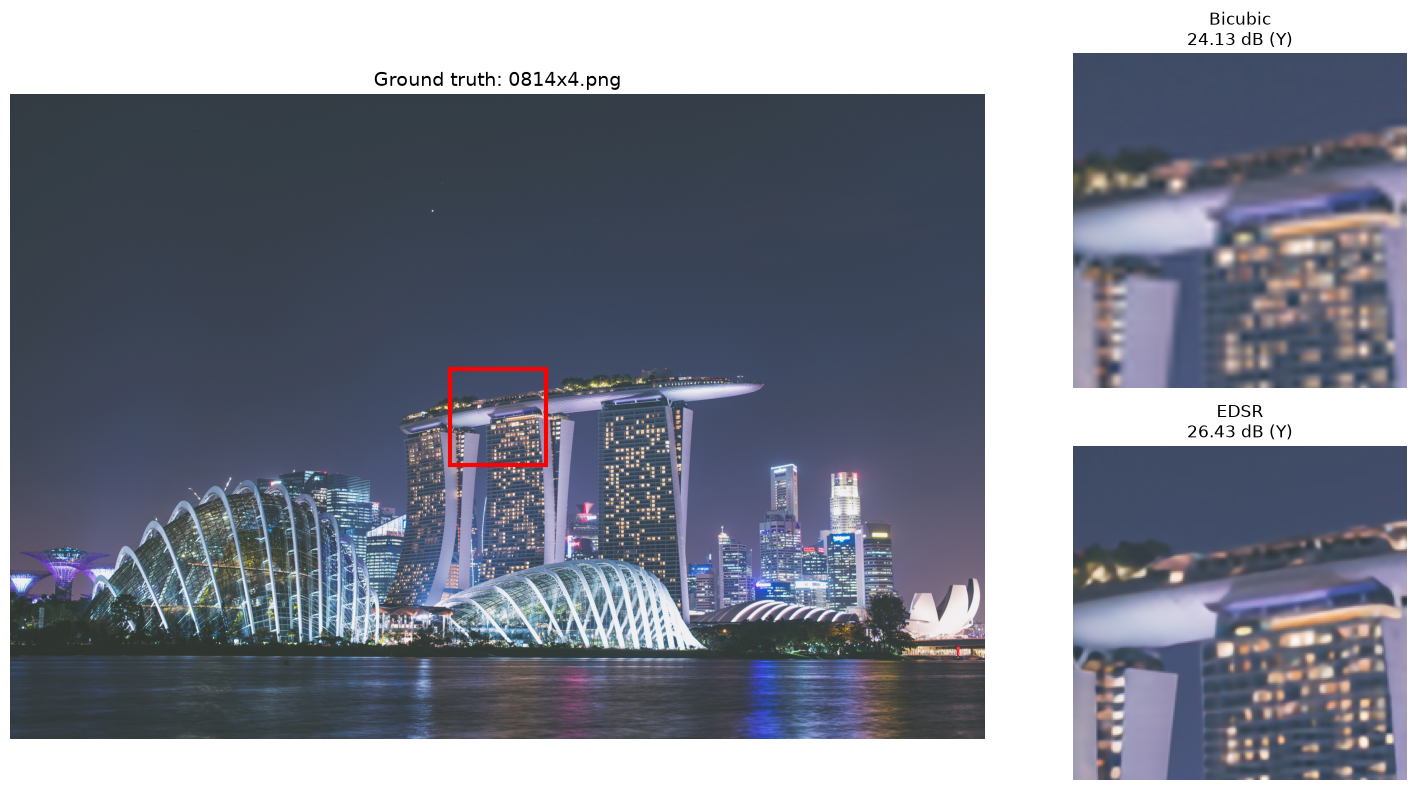
\includegraphics[width=0.66\textwidth]{newimg/0814.png} 
    \caption{\textbf{Geometric Structures (Img 0814):} The Bicubic interpolation 
blurs the illuminated building facades, whereas the EDSR model preserves sharper window and roof
boundaries, resulting in an improvement of \textbf{+2.30 dB} in PSNR (24.13 to 26.43 dB on the crop shown).}
    \label{fig:visual_0814}
\end{figure}

We also observe improvements in high-frequency textures, as shown in Figure \ref{fig:visual_0843},
a close-up of the spiralling centre of a rose. The Bicubic baseline blurs the overlapping petal
edges into a single smooth gradient, while the EDSR model recovers the individual folds and the
sharp boundary between the lit and shadowed sides of each petal.


\begin{figure}[htbp]
    \centering
    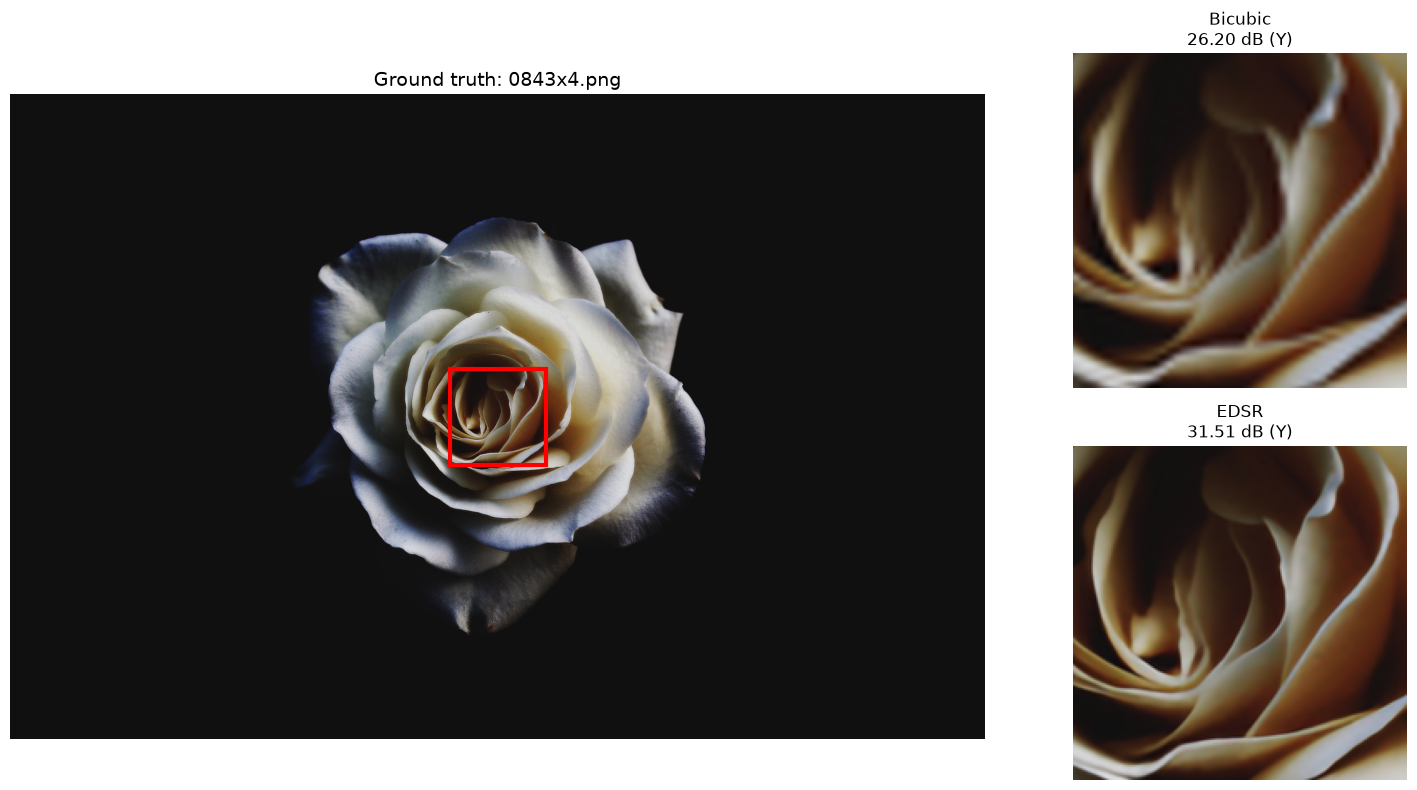
\includegraphics[width=0.66\textwidth]{newimg/0843.png} 
    \caption{\textbf{High-Frequency Textures (Img 0843):} In the Bicubic version the petal folds at the
centre of the rose merge into a smooth gradient. The EDSR model separates them again, resulting in an
improvement of \textbf{+5.31 dB} in PSNR (26.20 to 31.51 dB on the crop shown).}
    \label{fig:visual_0843}
\end{figure}

% ==================================================================
% 5. CONCLUSION AND LIMITATIONS
% ==================================================================
\section{Conclusion and Limitations}

We implemented Single Image Super-Resolution with the EDSR architecture, following
Lim et al.~\cite{lim2017}, and trained it for 100 epochs on the VUB ETRO GPU farm. On a test set
held out until the final evaluation it reaches 30.41~dB Y-PSNR, against 28.09~dB for bicubic interpolation, and it wins on SSIM and LPIPS as well. The $8\times$ self-ensemble adds a
further 0.07~dB at eight times the inference cost.

\subsection{Limitations and Observations}
Our results come with a number of caveats, and one of our own measurements points the wrong way.

\begin{enumerate}
    \item \textbf{Not everything we changed made things better.} The $8\times$ self-ensemble raises
    PSNR and SSIM but makes LPIPS worse, from 0.2804 to 0.2828. Averaging eight predictions pulls the
    output towards the mean of the plausible reconstructions, which is what a pixel-wise metric
    rewards and what a perceptual metric penalises. For eight times the inference cost we buy
    0.07~dB and lose a little perceptual quality, which is a bad trade outside a benchmark table.

    \item \textbf{We only model one kind of degradation.} Every low-resolution image we train and
    test on was produced by MATLAB bicubic downscaling. A real photograph that is simply small has
    been through sensor noise, compression and an unknown resampling filter. We have no evidence
    about how the model behaves on those, and we would expect it to do considerably worse.

    \item \textbf{More training would not rescue this.} The validation curve is close to flat over
    the last thirty epochs, so the model has essentially converged. What limits the result is the
    capacity of the network and the size of the training set, not how long we ran it. Getting a
    materially better number means changing the architecture or training on more data, which is the
    experiment we deliberately did not run this time.

    \item \textbf{One run, one seed, no error bars.} We trained each configuration once. That is
    enough to separate 28.09 from 30.41, but it is not enough to say that the 0.07~dB from the
    self-ensemble is real rather than noise.

    \item \textbf{The validation set is small.} Ten images are enough to rank checkpoints, but the
    peak of 31.27~dB on that set should not be read as a performance estimate. The test-set number
    is the one that means anything.

    \item \textbf{The model is heavy.} The residual body and the self-ensemble make inference far
    slower than interpolation, which rules this out for real-time use such as live video upscaling
    without further work on quantization or distillation.
\end{enumerate}

% ==================================================================
% REFERENCES
% ==================================================================
\begin{thebibliography}{99}

\bibitem{timofte2014}
Timofte, R. et al. “A+: Adjusted Anchored Neighborhood Regression for Fast Super-Resolution.” ACCV (2014).

\bibitem{dong2014}
Dong, C. et al. “Image Super-Resolution Using Deep Convolutional Networks.” IEEE TPAMI (2014).

\bibitem{kim2016}
Kim, Jiwon et al. ``Accurate Image Super-Resolution Using Very Deep Convolutional Networks.'' 2016 IEEE Conference on Computer Vision and Pattern Recognition (CVPR) (2016): 1646--1654.

\bibitem{lim2017}
Lim, B. et al. “Enhanced Deep Residual Networks for Single Image Super-Resolution.” CVPR Workshops (2017).

\end{thebibliography}

\end{document}